\documentclass[12pt,a4paper]{article}
 

% ---------------- PAQUETES ----------------
\usepackage[spanish, shorthands=off]{babel}
\usepackage[utf8]{inputenc}
\usepackage[T1]{fontenc} 
\usepackage{csquotes}
\usepackage{enumitem}
\usepackage{graphicx}
\usepackage{geometry}
\usepackage{setspace}
\usepackage{tocloft}
\usepackage[hidelinks]{hyperref}
\usepackage{pgfplots}
\usepackage{tikz}
\usepackage{amsmath}
\usepackage{microtype}
\usepackage{titletoc}
\usepackage{longtable}
\usepackage{booktabs}
\usepackage{multirow}
\usepackage[style=apa, backend=biber]{biblatex}

\addbibresource{references.bib} 
\pgfplotsset{compat=1.18}
\geometry{margin=2.5cm}
\setcounter{tocdepth}{2}
\onehalfspacing{}
\setlength{\parskip}{1em}


\begin{document}

% ---------------- PORTADA ----------------
\begin{titlepage}
    \centering
    \begin{flushleft}
        % 
\includegraphics[width=0.20\textwidth]{imagenes/logo_tec.png}
    \end{flushleft}

    {\large \textbf{Tecnológico Nacional de México Campus Culiacán}}\\[1.5cm]
    {\large Obsolescencia Programada: Cómo Erradicarla a Través de la Honestidad\\
    y Veracidad de la Información en Smartphones y Laptops\\
    Mediante los Principios de la Economía Circular}\\[1cm]
    {\large Ma. Aracely Martínez Amaya}\\[0.5cm]
    {\large Taller de Investigación I}\\[0.5cm]
    {\large \today}
\end{titlepage}

% ---------------- ÍNDICE ----------------
\tableofcontents
\newpage

% ---------------- SECCIONES ----------------
\section{Glosario}

\begin{description}
    \item[Obsolescencia Programada] Práctica de los fabricantes que consiste en diseñar un dispositivo con una vida útil limitada a propósito.
    \item[RAEE] Residuos de Aparatos Eléctricos y Electrónicos.
    \item[OCDE] Organización para la Cooperación y el Desarrollo Económicos.
    \item[GTIN] Número Global de Artículo Comercial.
    \item[TCO] Confederación Sueca de Empleados Profesionales.
    \item[GS1] Estándares Globales 1.
    \item[INEGI] Instituto Nacional de Estadística y Geografía. 
\end{description}

\newpage

\section{Antecedentes}

La obsolescencia programada es un problema que no solo afecta a los
consumidores, sino que perjudica directamente al medio ambiente debido a la
cantidad de recursos utilizados en la fabricación de productos —especialmente
electrónicos—, así como el desperdicio de muchos otros que son vistos como ``no
funcionales'' y, por lo tanto, son desechados. En 2023 se reportaron alrededor
de 6.92 mil millones de usuarios de teléfonos inteligentes en el mundo.
Considerando que el ciclo de vida promedio de estos dispositivos es de
aproximadamente 3 años, esto significa que se reemplazan constantemente, lo cual
genera una cantidad alarmante de residuos electrónicos. Además, esta cifra ni
siquiera toma en cuenta la explotación de materias primas que su producción
requiere desde el inicio de la cadena de suministro \parencite[p.~220]{ozturkcan2023}.

Según datos reportados en 2016, los Residuos de Aparatos Eléctricos y
Electrónicos (RAEE) alcanzaron aproximadamente 10.1 millones de toneladas en la
Unión Europea, lo que representó un incremento del 2.9\% respecto al año
anterior \parencite[p.~728]{malinauskaite2021}. En México, ese mismo año se
reportaron 998 mil toneladas de RAEE, siendo uno de los principales países que
generan estos residuos, ocupando el segundo lugar después de Brasil
\parencite[p.~207]{munoz2023}. Mientras la producción de equipos electrónicos
continúa en aumento, la vida útil de estos dispositivos sigue disminuyendo, lo
que inevitablemente amplifica la cantidad de residuos generados.

Se ha documentado que aproximadamente el 80\% de la contaminación y el 90\% de
los costos de fabricación asociados a los equipos electrónicos son consecuencia
de decisiones tomadas en la etapa de diseño del producto —precisamente donde
opera la obsolescencia programada \parencite[p.~728]{malinauskaite2021}. Además,
los residuos electrónicos contienen toxinas permanentes como arsénico, cadmio y
sustancias radiactivas, las cuales representan un riesgo grave para la salud de
las comunidades cercanas a los sitios de disposición, pudiendo incluso provocar
enfermedades de transmisión por el aire.

El impacto de este problema no se limita a las fronteras de los países
desarrollados. A pesar de que la exportación de residuos electrónicos con
sustancias tóxicas desde la Unión Europea hacia países no pertenecientes a la
Organización para la Cooperación y el Desarrollo Económicos (OCDE) es ilegal,
los países europeos envían cada año aproximadamente 352,474 toneladas métricas
de residuos electrónicos a naciones en vías de desarrollo, trasladando así las
consecuencias ambientales y sanitarias hacia las poblaciones más vulnerables
\parencite[p.~728]{malinauskaite2021}.

Allí, en lugares con pocos recursos y regulaciones débiles, estas comunidades
procesan los desechos de forma artesanal: incineran cables para recuperar cobre
y emplean ácidos para extraer metales preciosos de las placas. Esto contamina el
suelo, el agua y el aire, exponiendo a las personas a toxinas peligrosas. Lo que
se origina como una decisión de consumo en un país desarrollado termina
convirtiéndose en un problema de salud para comunidades vulnerables en otras
partes del mundo \parencite[p.~119]{unctad2024}.

La deshonestidad corporativa se ha intensificado con el tiempo, en parte porque
beneficia a aquellas empresas cuyo funcionamiento depende de prácticas nocivas
para la sociedad. Esto se sostiene a través de dos problemáticas: la sobrecarga
de información y el greenwashing; que permiten la persistencia de la
obsolescencia programada al aprovecharse del desinterés actual de la sociedad
para buscar información.

En estudios cualitativos realizados \parencite[p.~9]{holloway2025}, la
sobrecarga de información fue señalada por el 62\% de los participantes como uno
de los principales desafíos al momento de interpretar la extensa cantidad de
datos que las empresas divulgan sobre sus cadenas de suministro. De manera
similar, el 56\% expresó frustración ante la dificultad de acceder a información
transparente y verificable por parte de las marcas. El greenwashing tiene
relación con esta última cifra, pues ha sido señalado como una fuente principal
de escepticismo. Esta práctica —mediante la cual las empresas exageran o
tergiversan sus esfuerzos en materia de sustentabilidad— elimina la confianza
del consumidor. 

En el mercado existen aplicaciones que permiten obtener información detallada
sobre los productos:

\begin{itemize}
    \item \textbf{BARCODE LOOKUP:} Aplicación que, al escanear el código de
    barras de un producto, proporciona información técnica del mismo de forma
    inmediata, como especificaciones, características y datos relevantes del
    artículo.
    \item \textbf{GS1:} Base de datos que almacena y gestiona información
    técnica del producto junto con datos del fabricante, tales como lugar de
    fabricación, materiales utilizados en su elaboración y asociaciones con
    otras empresas.
    \item \textbf{ShopSavvy:} Aplicación móvil que permite escanear el código de
    barras de un producto, mostrando opiniones de usuarios que han adquirido
    dicho producto anteriormente.
\end{itemize}

Estas proporcionan un vistazo en el estado del mercado actual dentro del
contexto que se ha estado abordando: fuentes de información actuales que
permiten al consumidor conocer sobre los artículos que espera adquirir, así como
de sus fabricantes. 

La Gran Depresión fue un evento económico mundial originado en Estados Unidos
que provocó el inicio de varios fenómenos —como nuevas teorías económicas,
políticas macroeconómicas y cambios en instituciones económicas—. Uno de estos
fenómenos que ha influido, hasta la actualidad, en las tendencias de compra de
los consumidores es la obsolescencia programada —cuya primera aparición data en
1932 por Bernard London—como propuesta a las empresas para fomentar un mayor
consumismo por parte de la sociedad \parencite[p.~3]{corrocher2025}. La
propuesta definía un diseño deliberado de productos de tal manera que estos
tuvieran ciclos de vida más cortos con el propósito de crear una economía más
dinámica al estimular la demanda de nuevos productos, puesto que anteriormente
estos se vendían con la intención de que duraran décadas o incluso toda una vida
\parencite[p.~723]{malinauskaite2021}.

Esta práctica ha sido objeto de estudio por parte de numerosos expertos, quienes
buscan impulsar iniciativas que reduzcan el impacto ambiental y económico
generado por el consumo excesivo de productos. Entre estas iniciativas destaca el
movimiento right-to-repair —derecho a reparar—, el cual promueve que los
consumidores tengan acceso a las herramientas, piezas y conocimientos necesarios
para reparar sus propios productos, en lugar de reemplazarlos.

El movimiento right-to-repair es un movimiento moderno que ha tenido auge en
años recientes, puesto que cada vez más empresas —especialmente del sector
electrónico, industrial y automotriz— diseñan sus productos de manera que
resulten difíciles o imposibles de examinar y reparar sin herramientas
propietarias inaccesibles para el público general. Tiene como propósito
devolverle la autonomía al consumidor sobre los productos que adquiere,
exigiendo que las empresas ofrezcan acceso a piezas de repuesto a precios justos
y razonables en el mercado. En el contexto de los dispositivos electrónicos, el
movimiento también impulsa una mayor transparencia por parte de los fabricantes,
quienes deberían comunicar claramente el grado en que sus productos pueden ser
reparados. Esto permitiría a los consumidores tomar decisiones de compra más
informadas, considerando no solo el precio o las características del
dispositivo, sino también su viabilidad de reparación a largo plazo
\parencite{biscontini2024}.

Una de las primeras iniciativas dentro del movimiento right-to-repair fue el
sitio estadounidense iFixit —negocio establecido en 2003 en California,
EE.\@UU.—, el cual ofrecía manuales de reparación gratuitos especialmente para
dispositivos electrónicos. En respuesta a la creciente presión, algunas marcas
reconocidas comenzaron a establecer sus propios programas oficiales de
reparación, aunque con resultados cuestionables
\parencite[p.~220]{ozturkcan2023}.  

En 2022, Apple lanzó su programa Self-Service Repair, que otorgaba a los
usuarios acceso a documentación técnica para reparar sus dispositivos. Sin
embargo, la experiencia resultó lejos de ser conveniente para el usuario
promedio: los kits de reparación incluían piezas innecesarias para tareas
simples de reparación, así como instrucciones complejas que solo lograban
confundir a los consumidores. El resultado fue claro, parecía que la empresa no
quería que los consumidores fueran capaces de reparar por su propia cuenta,
dejando en evidencia que la iniciativa estaba lejos de representar un compromiso
real con el movimiento \parencite[p.~221]{ozturkcan2023}.

Ese mismo año, Samsung se asoció con iFixit para lanzar un programa similar que
permitía a algunos usuarios adquirir piezas de repuesto y acceder a guías de
reparación. No obstante, el programa excluía los dispositivos más recientes de
la marca y cubría únicamente un número limitado de reparaciones, lo que fue
percibido como un avance insuficiente, aunque al menos orientado en la dirección
correcta \parencite[p.~221]{ozturkcan2023}.

Estos ejemplos revelan una tendencia preocupante: mientras el discurso
corporativo adoptaba el lenguaje del movimiento, las implementaciones reales
seguían presentando barreras que, de forma sutil, continuaban incentivando al
consumidor promedio a optar por adquirir un producto nuevo antes que reparar el
que ya tenía. 

El movimiento right-to-repair es una de las iniciativas que no sólo toman en
cuenta el derecho del consumidor sobre los productos que adquiere, sino que
aborda un problema más amplio: el consumismo desmedido que caracteriza a la
sociedad actual, donde la explotación de recursos naturales, así como el
desperdicio que este provoca, es una de las muchas preocupaciones para el
desarrollo sustentable. En este sentido, el movimiento se alinea de manera
natural con los principios de la economía circular —un modelo que busca, en
palabras de \textcite[p.~229]{kirchherr2017}, alcanzar el desarrollo sustentable
mediante la creación simultánea de calidad ambiental, prosperidad económica y
equidad social, en beneficio de las generaciones presentes y futuras. La
economía circular propone cerrar el ciclo de vida de los productos mediante el
reciclaje, la reutilización y la reparación, devolviendo los bienes al mercado y
reduciendo así el impacto ambiental. 

Esta visión fue adoptada por la Comisión Europea en 2015, cuando lanzó su primer
Plan de Acción de Economía Circular bajo el principio de que ``nada debe
desperdiciarse'' buscando mejorar la economía global a través de un crecimiento
sustentable. Sin embargo, alcanzar estos objetivos resulta incompatible con la
obsolescencia programada, cuya lógica contradice directamente los fundamentos de
la economía circular, por lo que, para lograr sus objetivos principales, es
necesario primero regular —o contrarrestar— la obsolescencia programada
\parencite[p.~729]{malinauskaite2021}.

Entender el problema de la obsolescencia programada en la actualidad requiere ir
más allá de concebirla como una simple estrategia para acortar la vida útil de
los productos —el asunto es considerablemente más complejo. Los dispositivos
electrónicos no quedan obsoletos únicamente porque un componente falla. Más
bien, pierden funcionalidad por decisiones que toman los fabricantes mucho
después de que el producto fue adquirido. El problema actual no es que la
tecnología se desgaste, sino que las empresas han construido un sistema donde el
control sobre el dispositivo permanece en sus manos, incluso cuando el
consumidor ya lo pagó. 

Anteriormente, reparar un teléfono podía ser tan sencillo como cambiar una
pantalla o una batería con herramientas básicas. Sin embargo, los fabricantes
han implementado una práctica denominada “emparejamiento de piezas” o parts
pairing \parencite[p.~105]{alfieri2023}. Esto implica que cada componente
importante —como la pantalla, la batería o la cámara— posee un serial único que
debe coincidir con el de la placa principal del dispositivo. Si un usuario o
técnico independiente reemplaza una pieza, el sistema operativo la rechaza;
pudiendo mostrar mensajes de error, desactivar funciones específicas o, en casos
extremos, impedir el funcionamiento correcto del dispositivo. 

Todo este ciclo de reemplazo acelerado tiene una consecuencia muy visible: la
cantidad de residuos electrónicos crece de manera sostenida. Entre 2010 y 2022,
los desechos de pantallas, computadoras y equipos de telecomunicaciones
aumentaron un 30\% a nivel mundial, pasando de 8.1 a 10.5 millones de toneladas
\parencite[p.~108]{unctad2024}. Millones de teléfonos, computadoras son
descartados cada año, a pesar de que muchos aún podrían funcionar o ser
reparados. 

Además, la demanda de minerales necesarios para fabricar estos dispositivos
continúa en aumento. Materiales como el litio y el cobalto, esenciales para las
baterías, son cada vez más escasos y su extracción conlleva un elevado costo
ambiental y social. Se estima que para el año 2050 la necesidad de estos
minerales podría incrementarse hasta un 500\% \parencite[p.~41]{unctad2024}. En
otras palabras, se están consumiendo recursos de disponibilidad limitada para
fabricar productos que deliberadamente tienen una vida útil reducida. 

Ante este panorama, la presente investigación propuso diseñar una aplicación que
centralice datos técnicos y de sostenibilidad de productos electrónicos, con el
fin de que los usuarios puedan acceder a información real sobre la durabilidad,
costos de producción y opciones de reparación de sus dispositivos, contribuyendo
así a una toma de decisiones más informada y responsable. 

En conclusión, el consumidor requiere fuentes de información confiables que le
permitan tomar decisiones alineadas no solo con sus necesidades de consumo, sino
también con un mejor entendimiento de las prácticas corporativas que
habitualmente no son comunicadas de forma transparente. Esta información —para
que sea verdaderamente útil— debe presentarse de manera accesible, priorizando
la comprensión por encima de la exhaustividad, sin saturar al usuario con
terminología técnica o datos difíciles de interpretar. Asimismo, resulta
importante darle la oportunidad al consumidor de extender la vida útil de sus
dispositivos mediante la reutilización o la reparación, como alternativas
viables al reemplazo inmediato. 

En este contexto, si bien plataformas como BARCODE LOOKUP, GS1 o ShopSavvy son
referencias relevantes en materia de información de productos, su existencia
deja en claro un vacío tecnológico actual: la falta de una aplicación que
centralice información relevante sobre dispositivos electrónicos y sus
fabricantes, orientada específicamente a facilitar la toma de decisiones del
consumidor desde una perspectiva responsable. Es precisamente este vacío
tecnológico que el presente proyecto abordó, mediante el diseño de una
aplicación móvil que, a partir del escaneo del código de barras de un
dispositivo electrónico, permite al consumidor acceder de forma inmediata a
información sobre el producto y su fabricante, incluyendo criterios de
sostenibilidad, reputación corporativa y responsabilidad.
\newpage

\section{Planteamiento del Problema}

El mundo actual se distingue por la aceleración con la que se vive, lo que no
solo provoca un avance tecnológico cada vez mayor, sino que además trae consigo
la aparición de nuevos productos cuyo objetivo es resolver ``necesidades'' de la
sociedad; sin embargo, muchas de estas necesidades no son reales, sino que —en
palabras de \textcite[p.~347]{martinez2016}— son generadas por la maquinaria
publicitaria para inducir al consumidor a adquirir nuevos modelos antes de que
sea realmente necesario, manteniéndolo en un ciclo de consumo desmedido que
incrementa la demanda y, con ella, el uso de recursos.

Tomando en cuenta lo anterior, el consumidor promedio se ve envuelto en una
sobrecarga de información en donde lo único que conoce son las necesidades
impuestas por el capitalismo moderno; deja de estar interesado en lo que
conlleva la creación de un producto, buscando lo que aparentemente cumple con lo
que el consumidor busca, pues las campañas de marketing muestran únicamente lo
que las empresas quieren que el consumidor vea, lo que no siempre concuerda con
la realidad, generando confusión sobre la calidad técnica de un producto.
Además, la cantidad de información que un producto suele tener en sus fichas
técnicas suele provocar que, al vivir en una época de inmediatez, el consumidor
no se permita el tiempo de leer —o informarse— a profundidad. 

Además de los problemas que la inmediatez del mundo actual general, el
confinamiento debido a la pandemia COVID-19 tuvo sus propias consecuencias
dentro de la problemática del consumismo, donde muchas personas encontraron
refugio para sobrellevar el aislamiento a través de las compras en línea. Este
comportamiento se vio reflejado directamente en la cantidad de usuarios nuevos
en aplicaciones e-commerce; solo en 2019, el uso de los medios digitales
incremento un 24\% en relación con el 2017 en México, con un valor de 491
millones de pesos \parencite[p.~123]{bejar2023}. El hecho de comprar en línea
resultó una actividad sencilla para el consumidor, sin requerir ningún tipo de
esfuerzo, por lo que millones de personas comenzaron a unirse a este tipo de
actividad sin realmente tener un objetivo en sus compras. 

La problemática del consumismo tiene múltiples causas; sin embargo, la actual
investigación estará enfocada principalmente en dos estrategias empleadas por
las empresas para mantenerlo. El uso del llamado greenwashing —la práctica de
presentar productos y campañas de marketing como ecológicos o sostenibles sin
serlo realmente— genera una percepción de responsabilidad ambiental que es, en
esencia, engañosa. Así como la sobreabundancia de información que confunde al
consumidor, desalentando cualquier interés por conocer a fondo la composición o
el impacto real de lo que adquiere. Ambas estrategias, combinadas con la
obsolescencia programada —el diseño deliberado de productos con una vida útil
limitada—, garantizan que el ciclo del consumismo se mantenga activo de forma
ininterrumpida, sin que el consumidor encuentre un momento de pausa para
cuestionar sus hábitos de compra. 

Con base en lo anterior, la presente investigación busca responder a la
siguiente pregunta: \noindent\textit{¿Cómo puede una aplicación móvil de escaneo
de código de barras contribuir a reducir la asimetría de información en la
compra de productos electrónicos (smartphones y laptops) y fomentar un consumo
más informado y sostenible?}
\newpage

\section{Objetivos}

\subsection{General}

Desarrollar una aplicación móvil con una arquitectura de información
basada en la divulgación progresiva que centralice la información más relevante
obtenida de diversas bases de datos vinculadas a los códigos de barras de
productos electrónicos, específicamente smartphones y laptops, con el propósito
de fomentar en el consumidor el desarrollo de hábitos de consumo responsable. 

\subsection{Específicos}

\begin{enumerate}
    \item Identificar el tipo de información obtenida a través de bases de datos
    vinculadas a códigos de barras de dispositivos electrónicos, específicamente
    smartphones y laptops.
    \item Analizar la información obtenida en el objetivo anterior desde la
    perspectiva del consumidor.
    \item Implementar una base de datos que estructure y almacene la información
    recopilada durante el proceso de investigación.
    \item Desarrollar una aplicación móvil con una arquitectura de información
    basada en el principio de divulgación progresiva que minimice la carga
    cognitiva del usuario respecto a los datos técnicos de los productos.
    \item Diseñar e implementar pruebas de software que garanticen el
    comportamiento esperado de la aplicación.
    \item Realizar pruebas de campo para evaluar el nivel de aceptación de la
    aplicación por parte de los usuarios, con el propósito de identificar
    oportunidades de mejora en la experiencia de uso.
\end{enumerate}

\newpage

\section{Justificación}

En la actualidad, un número creciente de personas manifiesta preocupación por el
medio ambiente y aspira a consumir de manera más responsable. Sin embargo, el
mercado no facilita esta tarea. En primera instancia, se encuentra el
greenwashing, práctica mediante la cual las empresas emplean un lenguaje
vagamente ecológico para aparentar sostenibilidad sin serlo realmente. Mensajes
sobre ``compromiso con el planeta'' o ``materiales reciclados'' frecuentemente
encubren productos que siguen siendo difíciles de reparar y de vida útil
reducida. Esto genera desconfianza: el consumidor no sabe en quién confiar
\parencite[p.~9]{holloway2025}.

A esto se suma la sobrecarga de información. Entre datos técnicos complejos,
especificaciones confusas y campañas de marketing, resulta muy difícil para el
consumidor determinar qué producto es realmente duradero. La ausencia de
estándares claros sobre reparabilidad o durabilidad hace que, aunque la
intención de consumir de forma sostenible exista, la falta de herramientas para
hacerlo termine perpetuando el mismo ciclo: adquirir, usar brevemente,
reemplazar \parencite[p.~9]{holloway2025}.

Frente a esta problemática, la economía circular surge como un marco regulatorio
orientado a contrarrestar precisamente lo que este ciclo de consumo acelerado
genera: el desperdicio desmedido de recursos. En México, aunque esta idea de
economía circular es relativamente nueva, en años recientes ha incrementado el
interés por adoptarla mediante leyes que aún están en discusión. Sin embargo,
existen normas oficiales que, aunque no es su objetivo principal, encaminan al
país a su adopción \parencite[p.~220]{munoz2023}:

\begin{itemize}
    \item \textbf{NOM-052-SEMARNAT-2005:} Establece las características, el
    procedimiento de identificación, clasificación y los listados de los
    residuos peligrosos.
    \item \textbf{NOM-161-SEMARNAT-2011:} Establece los criterios para
    clasificar los Residuos de Manejo Especial y determinar cuáles están sujetos
    a Plan de Manejo.
\end{itemize}

Si bien estas normas representan un avance en la gestión de residuos, buscando
reducir su impacto ambiental, su enfoque se limita al manejo posterior de los
mismos, sin abordar una de las principales causas que los genera: la
obsolescencia programada. 

Es precisamente en este vacío donde se situó el enfoque central de la
investigación. En la actualidad, las empresas comercializan sus productos con
acceso asimétrico a la información: mientras los fabricantes conocen en detalle
la calidad, los riesgos y las limitaciones de sus productos, esta información
raramente es comunicada al consumidor de forma completa o comprensible. Esto
constituye una práctica que perjudica directamente al consumidor, quien toma
decisiones de compra sin contar con los elementos necesarios para evaluarlas con
criterio. Ante esto, la aplicación buscó reducir esta brecha
informativa centralizando, de manera accesible, datos relevantes sobre
durabilidad, reparabilidad, prácticas corporativas de los dispositivos
electrónicos. De esta forma, no solo se combate la desinformación que favorece a
la obsolescencia programada, sino que también se le otorga al consumidor una
herramienta para identificar el greenwashing y navegar en la información con mayor
claridad, fomentando así decisiones de consumo más conscientes y responsables. 

A fin de garantizar la viabilidad del proyecto, se establecieron una serie de
delimitaciones que permitieron mantener un enfoque claro acorde con las
capacidades actuales dentro del contexto de la materia. La investigación se
restringió a productos electrónicos, específicamente smartphones y laptops. En
ambas categorías se abordaron las marcas Apple, Samsung, Huawei y Xiaomi, dado
que representan mayor presencia en el mercado; además, constituyen un sector
donde la información sobre reparaciones suele ser especialmente restrictiva. 

La recolección de datos se limitó a información disponible dentro de
México, llevando a cabo un estudio transversal que permitió analizar el estado
actual de la problemática en el país. Debido a que un análisis de alcance global
implicaría una cantidad de tiempo que exceden los límites del presente proyecto
se eligió la anterior delimitación geográfica. Asimismo, la cantidad de
información manejada se acotó, priorizando aquellos datos más relevantes
para el consumidor, con el fin de garantizar que el diseño se mantenga dentro de
las capacidades técnicas disponibles. 

\newpage

\section{Marco Teórico}

La obsolescencia programada está definida como “el uso de técnicas mediante las
cuales una entidad responsable de lanzar un producto en el mercado busca reducir
el ciclo de vida útil —de manera deliberada— de dicho producto”
\parencite[p.~741]{malinauskaite2021}. Esta se manifiesta de distintas formas.
Una de ellas consiste en diseñar productos difíciles o imposibles de reparar, ya
sea porque las piezas necesarias no están disponibles en el mercado o porque el
costo de la reparación resulta tan elevado que adquirir uno nuevo termina siendo
la opción más práctica —no porque la reparación sea técnicamente imposible, sino
porque el fabricante decidió restringirla mediante limitaciones digitales
\parencite[p.~105]{alfieri2023}.

Según \textcite[p.~225]{kirchherr2017}, la economía circular “describe un
sistema económico basado en modelos de negocio que sustituyen el concepto de
``fin de vida útil'' con el propósito de alcanzar un desarrollo sustentable”. En
la práctica, este modelo se sostiene sobre nueve principios fundamentales
—rechazar, replantear, reducir, reutilizar, reparar, restaurar, reciclar,
recuperar, reusar— orientados a generar calidad ambiental y prosperidad
económica.

Entre los principios de la economía circular, la reparación, restauración, así
como el replanteamiento resultan particularmente relevantes como estrategias
para contrarrestar la lógica de reemplazo acelerado que sustenta la
obsolescencia programada. Estos principios, según
\textcite[pp.~29-31]{lambiase2024} están definidos de la siguiente forma:  

\begin{enumerate}
    \item La \textbf{reparabilidad} de productos es un principio orientado a
    extender su vida útil mediante el mantenimiento. Su implementación en el
    mercado electrónico puede tomar dos vías: la intervención de talleres de
    reparación especializados con acceso a las piezas necesarias, o la
    reparación por parte del propio usuario, siempre que la información técnica
    y las herramientas requeridas sean accesibles. 
    \item La \textbf{restauración} implica reemplazar componentes viejos o
    desgastados por partes nuevas, extendiendo así la vida útil del producto.
    Este principio comparte con la reparabilidad una condición para su
    implementación exitosa: que las herramientas, piezas necesarias sean
    accesibles para quienes buscan llevarla a cabo. Sin embargo, también depende
    de decisiones tomadas desde la etapa de diseño —los productos deben
    diseñarse bajo un esquema modular que permita retirar, reparar, reemplazar
    sus componentes de forma sencilla. 
    \item FInalmente, el \textbf{replanteamiento del consumo} se materializa en
    el modelo ``product as a service'' —producto como servicio—, en el que la
    empresa retiene la propiedad del bien, ofreciendo al cliente únicamente su
    uso mediante arrendamiento, renta o pago por uso. Bajo este esquema, los
    fabricantes tienen un incentivo directo para diseñar productos más
    duraderos, lo que reduce el desperdicio asociado al reemplazo constante. 
\end{enumerate}

Sin embargo, el modelo de producción dominante actual opera en sentido
contrario, priorizando el consumo a corto plazo y llevando al planeta hacia una
situación cada vez más insostenible. Este ritmo de producción acelerado
—activamente sostenido por prácticas como la obsolescencia programada— resulta
incompatible con los fundamentos de la economía circular, lo que convierte su
regulación en una condición necesaria para alcanzar los objetivos que este
modelo propone. 

Otra variante es la obsolescencia tecnológica o de incompatibilidad, que ocurre
cuando la introducción de un producto técnicamente más avanzado vuelve obsoletos
los modelos anteriores —por ejemplo, mediante actualizaciones de software
incompatibles o tan voluminosas que obligan al usuario a adquirir una versión
más reciente del dispositivo \parencite[p.~724]{malinauskaite2021}. El usuario
se encuentra entonces con un dispositivo que físicamente funciona, pero que no
puede utilizarse para las tareas básicas de la vida diaria. La presión por
mantenerse conectado termina empujándolo a adquirir un modelo más reciente,
aunque el anterior aún sea funcional. 

Mientras que la obsolescencia programada es un fenómeno ocasionado
principalmente por la industria, los consumidores también juegan un papel
importante, puesto que la obsolescencia percibida fomenta el reemplazo
innecesario de productos completamente funcionales
\parencite[pp.~6-7]{corrocher2025}. Sin embargo, atribuir este comportamiento
únicamente a una decisión libre del consumidor sería simplista. La economía
conductual señala que las personas suelen tomar decisiones irracionales debido a
su ``racionalidad limitada'', lo que las hace susceptibles a ser manipuladas en
ciertos contextos \parencite[pp.~725-726]{malinauskaite2021}.

En el mercado de productos electrónicos, esto se traduce en una sobrecarga
cognitiva provocada por la cantidad, así como complejidad de la información
disponible, dificultando que el consumidor pueda comparar y evaluar sus opciones
de forma efectiva —un fenómeno conocido como ``confusopolio''. En este fenómeno,
el consumidor se ve saturado de información deliberadamente confusa que eleva
los costos cognitivos de búsqueda, dificultando su capacidad de tomar decisiones
de compra verdaderamente informadas. 

Frente a esta problemática de sobrecarga informativa, resulta importante
examinar las herramientas que actualmente existen para facilitar el acceso a
información sobre productos electrónicos. BARCODE LOOKUP representa una
aproximación a este problema mediante el escaneo del código de barras de
cualquier producto. Su base de datos internacional —que cuenta con más de mil
millones de productos registrados provenientes— permite al usuario obtener, de
forma inmediata, información como nombre del producto, fabricante, descripción e
imágenes. Adicionalmente, la plataforma vincula al usuario con los vendedores en
línea que comercializan el mismo artículo, facilitando la comparación de precios
entre distintas tiendas. Sus datos provienen de una red de más de 1,500
minoristas a nivel mundial, así como de contribuciones directas de usuarios, lo
que le permite mantenerse actualizada de forma continua. 

Otra herramienta orientada a reducir la sobrecarga informativa del consumidor es
ShopSavvy \parencite{shopsavvy2008}, una aplicación móvil disponible para iOS y
Android que permite escanear el código de barras de cualquier producto para
acceder a precios en tiendas locales. Sin embargo, su aportación más relevante
en el contexto del confusopolio es otra: la integración de opiniones de usuarios
reales. A diferencia de las especificaciones técnicas —cuya comprensión exige un
nivel de conocimiento que no todos los consumidores poseen—, las reseñas ofrecen
información basada en experiencia directa de uso, lo que permite evaluar el
rendimiento real de un producto sin necesidad de entender terminología
especializada. En un mercado donde la complejidad informativa es, en muchos
casos, deliberada, este tipo de evaluación colectiva representa una vía
accesible para que el consumidor tome decisiones más informadas y,
potencialmente, menos susceptibles a la manipulación que sustenta la
obsolescencia percibida. 

Asimismo, el greenwashing representa otra fuente de desinformación que
profundiza la confusión del consumidor. \textcite[p.~196]{font2025} lo define
como el uso indebido de la comunicación sustentable para engañar al consumidor
sobre las características sostenibles de un producto. Esta práctica resulta
especialmente problemática porque explota las expectativas legítimas del
consumidor, quien asume que una empresa con discurso ecológico implementa
programas ambientales reales, adopta iniciativas sociales, opera bajo criterios
de sostenibilidad económica. Cuando estas expectativas no corresponden a la
realidad, el resultado es un escepticismo generalizado que le dificulta al
consumidor distinguir entre marcas genuinamente responsables y aquellas que
simplemente lo aparentan. 

Ante este panorama de desconfianza generado por el greenwashing, GS1 representa
una fuente de datos que opera en sentido contrario: en lugar de comunicar lo que
las empresas quieren mostrar, gestiona información verificable sobre productos.
GS1 es una organización global sin fines de lucro presente en más de 150 países
que desarrolla y administra estándares internacionales de identificación de
productos —siendo el código de barras su herramienta más reconocida. A través de
su sistema de identificación único por producto, conocido como Número Global de
Artículo Comercial (GTIN), es posible acceder a datos sobre el origen de los
materiales, el proceso de fabricación las certificaciones de sostenibilidad
reales asociadas a un producto y su fabricante. Esta última función resulta
especialmente significativa: GS1 Sweden, en colaboración con TCO Certified
—organismo líder en certificación de sustentabilidad para productos de
tecnología— ha integrado el GTIN en sus procesos de certificación, permitiendo
que productos electrónicos desarrollados puedan ser rastreados y vinculados
directamente a sus certificaciones verificadas \parencite{gs12025}. Esto
convierte a GS1 en una herramienta con potencial para contrarrestar el
greenwashing, al ofrecer al consumidor un medio de verificación objetivo frente
a los discursos corporativos que no siempre corresponden a la realidad. 

En un contexto comercial donde este tipo de problemáticas influyen negativamente
en las decisiones de compra, toma especial importancia la existencia de fuentes
de información no solo confiables, sino presentadas de forma comprensible para
cualquier tipo de consumidor, independientemente de su conocimiento previo sobre
tecnología. La teoría de la riqueza de los medios sugiere que la cantidad
adecuada de información en un estímulo puede reducir la incertidumbre e influir
positivamente en el resultado de la comunicación \parencite[p.~197]{font2025}.
Sin embargo, este equilibrio es delicado: si bien una mayor riqueza informativa
transmite más datos al receptor, un exceso puede derivar en sobrecarga
informativa. Esta ocurre cuando los requerimientos de procesamiento de
información superan la capacidad del individuo para procesarla, convirtiéndose
en un obstáculo para la toma de decisiones incluso cuando dicha información es
relevante \parencite[p.~197]{font2025}.  

La situación se agrava cuando la información es poco familiar, compleja o
presentada a un ritmo mayor al que el receptor puede asimilarla —condiciones que
caracterizan precisamente la forma en que los fabricantes de dispositivos
electrónicos comunican sus productos al mercado. 

Frente a la problemática de sobrecarga informativa previamente descrita, la
divulgación progresiva —progressive disclosure— emerge como una estrategia de
diseño de interfaz orientada a mitigar sus efectos en la toma de decisiones del
consumidor. Este enfoque consiste en presentar inicialmente un conjunto reducido
de atributos clave, ofreciendo acceso opcional a información más detallada en
etapas posteriores. \textcite[pp.~15-19]{hu2022} demostraron empíricamente que
los usuarios expuestos primero a conjuntos simplificados de información logran
establecer criterios de decisión más estables, los cuales mantienen al
enfrentarse posteriormente a datos más complejos. En contraste, quienes reciben
toda la información de forma simultánea exhiben una mayor inconsistencia entre
sus preferencias declaradas y sus decisiones reales —fenómeno atribuido
directamente al exceso de carga cognitiva. Aplicado al contexto de dispositivos
electrónicos, este principio sugiere que una aplicación que estructure la
información técnica y ambiental de manera progresiva no solo reduciría la
confusión del consumidor, sino que favorecería decisiones de compra más
alineadas con sus valores y necesidades reales.

La aplicación diseñada toma como eje central el cuidado de la carga cognitiva
del usuario, adoptando la divulgación progresiva como estrategia
estructural de presentación de información, permitiendo que el consumidor
procese los datos de manera gradual, construya criterios de decisión sólidos
antes de enfrentarse a información de mayor complejidad. Así pues, se busca
que las decisiones de compra sean producto de una comprensión real, no de una
saturación informativa que, como se ha descrito, puede derivar en elecciones
incongruentes con las necesidades y valores del propio usuario. 

Además, la aplicación reconoce el valor de la experiencia colectiva como fuente de
información accesible. A diferencia de las especificaciones técnicas
—cuya interpretación exige conocimientos especializados—, las opiniones de
usuarios reales ofrecen una evaluación basada en el uso cotidiano del producto.
La plataforma integró este tipo de reseñas bajo un modelo libre de
patrocinios, con el fin de preservar su credibilidad, contrarrestando la
distorsión informativa que caracteriza los canales comerciales convencionales.
Finalmente, retomando la problemática de la obsolescencia programada, la aplicación
incorporó un directorio de opciones de reparación cercanas al usuario. Esta
funcionalidad busca traducir los principios de reparabilidad y restauración de
la economía circular —previamente descritos— en una herramienta que
fomente su adopción, contribuyendo así a la concientización del consumidor y a
la extensión de la vida útil de los dispositivos electrónicos.
\newpage

\section{Hipótesis}

¿Cómo puede una aplicación móvil de escaneo de código de barra contribuir a reducir 
la asimetría de información en la compra de productos electrónicos y fomentar un 
consumo más informado y sostenible? 

Mediante el desarrollo de una aplicación que centralice la información actualmente 
dispersa sobre productos electrónicos —con énfasis en smartphones y laptops— y sus 
fabricantes, se espera generar en el consumidor una reflexión crítica sobre sus propios
hábitos de consumo: que se cuestione cuáles son realmente sus necesidades como persona 
antes de asumirlas como necesidades de consumidor, pues identificar ese origen es el 
primer paso para tomar decisiones conscientes. 

Se espera que la herramienta impulse la adopción de principios de la economía circular, 
dotando al usuario de información suficiente para prevenir el desperdicio de tiempo y dinero. 
Esto implica que pueda evaluar la calidad real de un producto a partir de sus especificaciones 
técnicas y reseñas, compararlo con otras opciones disponibles en el mercado, y valorarlo según 
su comportamiento social y su capacidad de reparación. Este último factor —la reparabilidad— 
puede transitar de ser un aspecto técnico complejo y poco conocido a convertirse en un criterio 
accesible y popular; condición que amplía la diversidad de soporte disponible para el dispositivo 
y fortalece la posición del consumidor frente a la narrativa que las empresas construyen por conveniencia. 

Se espera que la aplicación permita que cualquier persona, con tan solo escanear el código 
de barras de un producto, acceda a información integral sobre el mismo. Esta no se limitará 
a sus especificaciones técnicas, sino que también incluirá datos relevantes sobre la empresa 
fabricante: sus sedes, certificaciones, alianzas comerciales y su compromiso real con el medio 
ambiente. Adicionalmente, la plataforma facilitará la localización de centros de reparación autorizados 
o cercanos al usuario, fomentando la reutilización de dispositivos y extendiéndoles una segunda vida 
útil. Por último, y como elemento vital, integrará reseñas de consumidores del producto: opiniones 
no patrocinadas, reales y conscientes. 

\newpage

\section{Bosquejo del Método}

\subsection{Población}

La presente investigación tomará como enfoque principal la población del
municipio de Culiacán, Sinaloa, México. De acuerdo con el último Censo de
Población y Vivienda realizado por el Instituto Nacional de Estadística y
Geografía \parencite[p.~23]{inegi2021}, Culiacán registra una población total de
1,003,530 habitantes, lo que representa el 33.2\% de la población total del
estado de Sinaloa.

Dentro de este universo, se delimitó como población de estudio a los habitantes
de 27 años de edad. Este grupo resulta de particular interés debido a que ha
transitado por las distintas etapas del comercio moderno: desde la adquisición
de productos exclusivamente a través de catálogos o tiendas físicas, hasta la
adopción de las compras en línea, cada una con estrategias de marketing propias.
Dicha trayectoria les otorga una perspectiva amplia frente al consumo de
cualquier tipo de producto. Asimismo, por tratarse de adultos en plena vida
laboral —y en la mayoría de los casos con los estudios concluidos—, es razonable
suponer que ya han adquirido los tipos de productos en los que se centra esta
investigación: laptops y smartphones. A esto se suma que una persona en esta
etapa de vida cuenta con mayor criterio, autonomía económica y experiencia
acumulada en decisiones de compra.

De acuerdo con el Censo de Población y Vivienda 2020, la población de Culiacán
correspondiente al rango de 27 años o más asciende a 578,109 habitantes. Este
dato es congruente con la edad mediana registrada por el propio INEGI para ese
año, que fue de 29 años; en efecto, el 50\% de la población total del municipio
equivale a:

\[
\frac{1{,}003{,}530}{2} = 501{,}765 \text{ habitantes}
\]

lo que confirma que más de la mitad de la población se concentra en edades
cercanas al rango de interés.

Con el fin de obtener una estimación más precisa para el año 2026, se incorporó
al cálculo la población que, en 2020, se encontraba en el rango de 20 a 24 años,
puesto que dichas personas habrán alcanzado los 27 años o más transcurridos seis
años. Al sumar este grupo al total anterior, se obtiene una base poblacional
ampliada de:

\[
578{,}109 + 88{,}495 = 666{,}604 \text{ habitantes}
\]

Además, para proyectar esta cifra a 2026, se descontó la mortalidad estimada del
periodo. Tomando como referencia un promedio de 18,902 defunciones anuales
registradas en Sinaloa a partir de 2020 \parencite{inegi_mortalidad}, y
considerando que Culiacán concentra el 33.2\% de la población estatal, le
corresponden aproximadamente:

\[
18{,}902 \times 0.332 \approx 6{,}275 \text{ defunciones anuales}
\]

Descontando estas defunciones acumuladas durante el periodo 2020--2026, la
población estimada en el rango de 27 años o más para el presente año es de:

\[
666{,}604 - (6{,}275 \times 6) = 666{,}604 - 37{,}650 \approx 628{,}954 
\text{ habitantes}
\]

\subsection{Muestra}

Tomando los valores anteriormente detallados para la población a estudiar, se
procedió a calcular el tamaño de muestra necesario. Empleando la fórmula
propuesta por \textcite[p.~75]{cochran1977}:
\[
n = \frac{\dfrac{t^2 PQ}{d^2}}{1 + \dfrac{1}{N}\left(\dfrac{t^2 PQ}{d^2} - 1\right)}
\]

\noindent con un nivel de confianza del 95\% ($t = 1.96$), una proporción
esperada de $P = 0.5$, y un margen de error de $d = 0.05$, se obtuvo:

\[
n = \frac{\dfrac{(1.96)^2 (0.5)(0.5)}{(0.05)^2}}{1 + \dfrac{1}{1{,}003{,}530}
\left(\dfrac{(1.96)^2 (0.5)(0.5)}{(0.05)^2} - 1\right)}
= \frac{384.16}{1 + \dfrac{383.16}{1{,}003{,}530}} \approx 384 \textrm{ encuestados}
\]

Posteriormente, aplicando la asignación proporcional por estrato
\parencite[p.~91]{cochran1977}, se determinó la muestra correspondiente al
segmento de habitantes de interés con respecto a la población total del
municipio:

\[
n_h = n \cdot \frac{N_h}{N} = 384 \cdot \frac{628{,}954}{1{,}003{,}530} 
\approx 241 \textrm{ encuestados}
\]

Por lo tanto, la muestra definitiva para esta investigación quedó establecida en
\textbf{241 encuestados}, representando de manera proporcional al segmento
poblacional de interés dentro del municipio de Culiacán, Sinaloa.

\subsection{Tipo de Estudio}

La presente investigación adopta un enfoque metodológico mixto. En primer lugar,
es de carácter documental, dado que su sustento teórico está construido a partir de
estudios/experimentos previos que respaldan los efectos positivos propuestos que
la disponibilidad de la información —presentados de forma adecuada— tiene 
en la toma de desiciones del consumidor.

Asimismo, la investigación integra un componente cuantitativo
y cualitativo mediante la aplicación de una encuesta —cuyo instrumento se
presenta en el Anexo A— dirigida a consumidores de dispositivos electrónicos.
Dicho instrumento tiene como propósito recabar la opinión de usuarios reales
respecto a sus hábitos de consumo, su acceso a información al momento de
adquirir un producto, así como la percepción de utilidad que tendría una herramienta
como la propuesta en este proyecto. La muestra representativa está conformada por
241 encuestados que permitirá obtener resultados con un nivel de confianza 
adecuado para validarla relevancia de la aplicación dentro del contexto estudiado.

\newpage

% \section{Arquitectura}

El sistema adoptará una \textbf{arquitectura cliente-servidor} con un backend
monolítico modular, implementando el patrón de diseño \textit{gateway
aggregation} con el objetivo de centralizar la lógica de integración con
múltiples fuentes externas.

El patrón gateway aggregation —mostrado en la
Figura~\ref{fig:gateway-aggregation}— consiste en utilizar un componente
intermediario que recibe una sola petición del cliente, la descompone en
múltiples llamadas a servicios backend, agrega los resultados y devuelve una
única respuesta.


\begin{figure}[h!]
    \centering
    \fbox{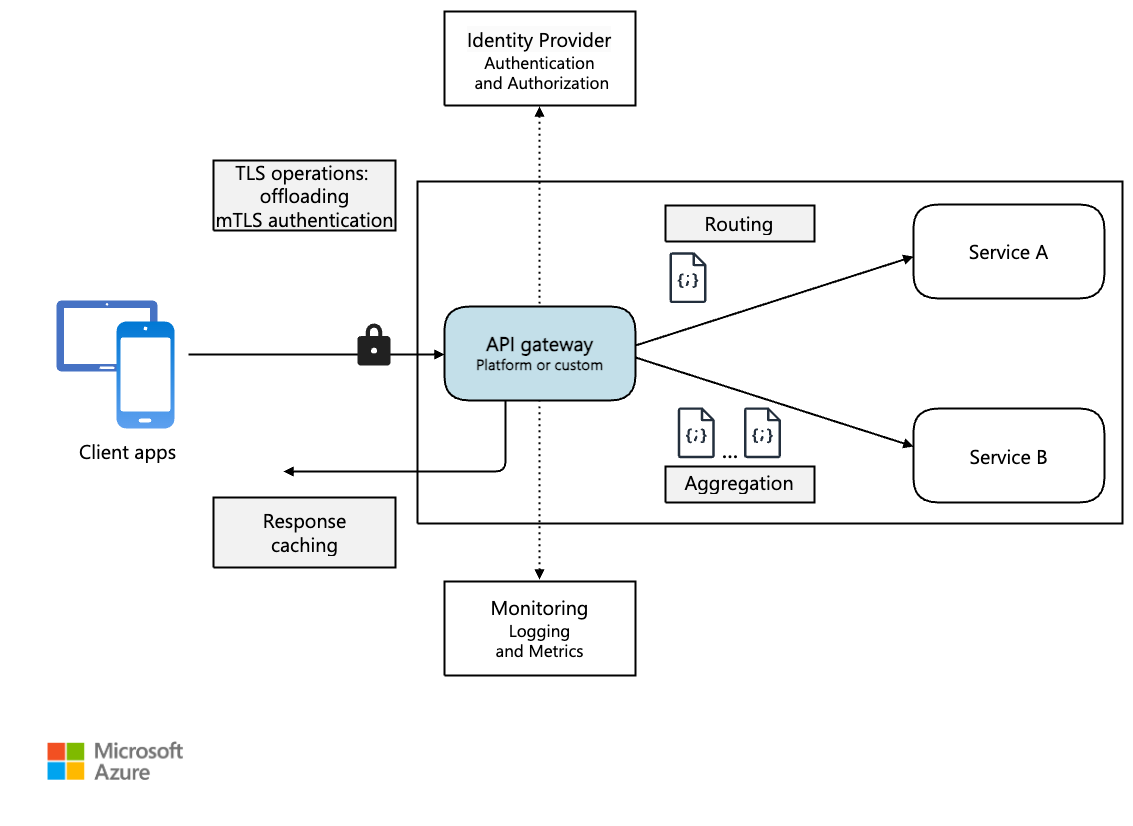
\includegraphics[width=0.8\textwidth]{imagenes/gateway-aggregation.png}}
    \caption{Gateway Aggregation}\label{fig:gateway-aggregation}
\end{figure}

\begin{figure}[h!]
    \centering
    \fbox{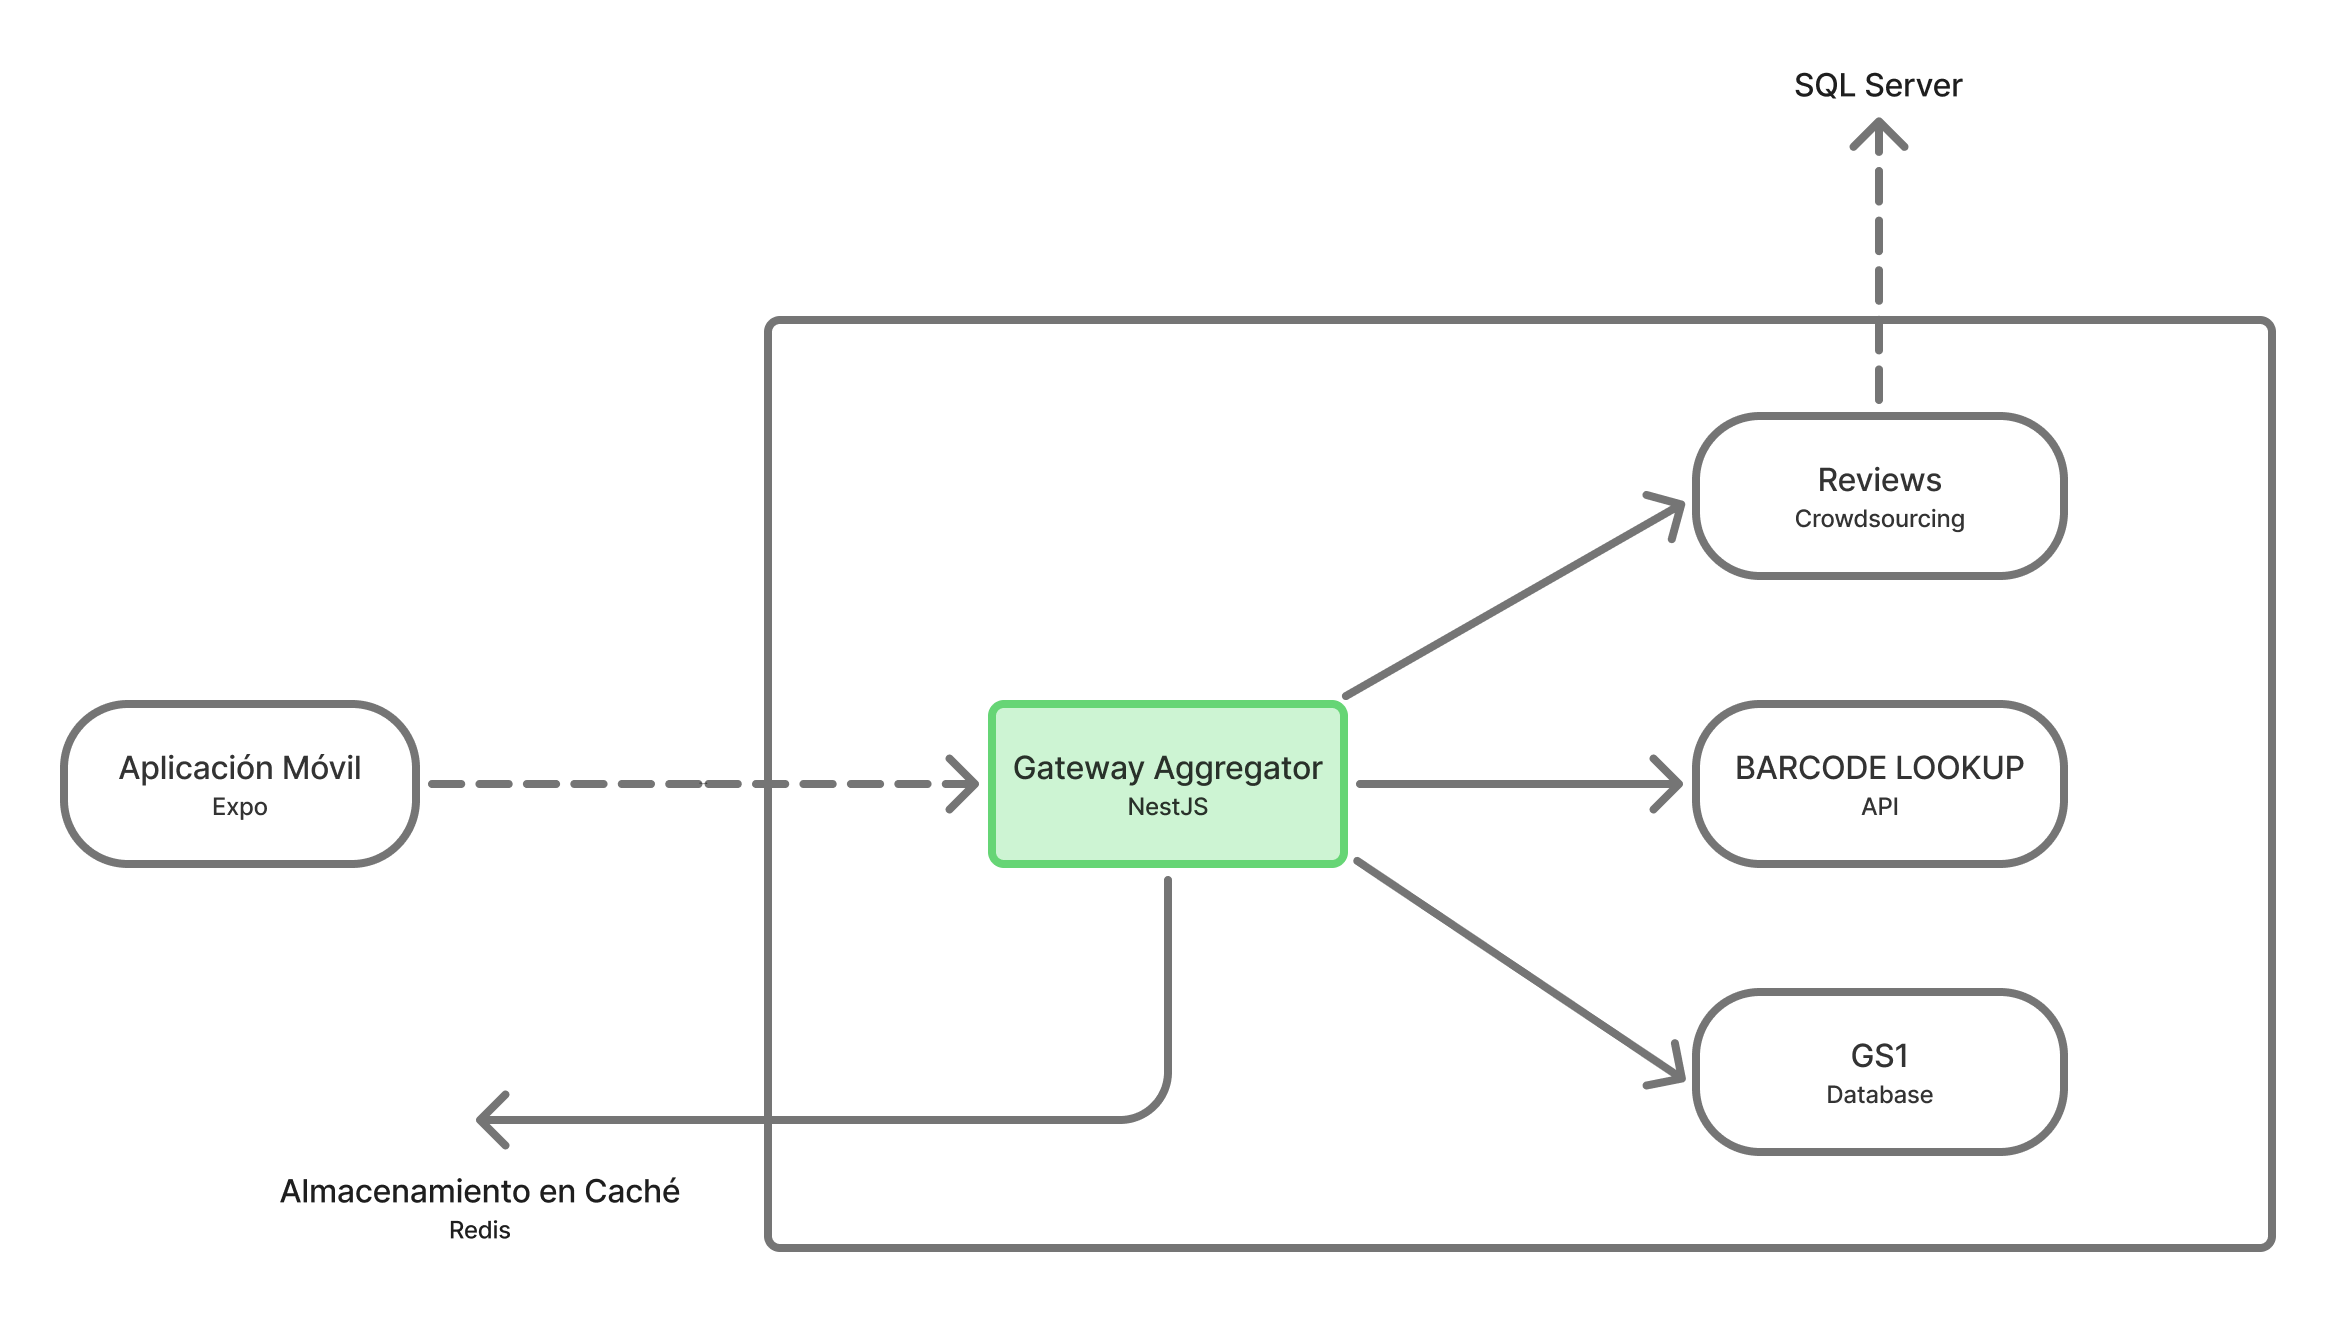
\includegraphics[width=0.8\textwidth]{imagenes/diagrama-sistema.png}}
    \caption{Diagrama del Sistema}\label{fig:diagrama-sistema}
\end{figure}
% \newpage

\section{Casos de Uso}

\subsubsection{CU-01: Escaneo de Producto}
Este caso de uso describe el proceso mediante el cual el usuario podrá escanear
el código de barras de un producto utilizando la cámara de su dispositivo móvil.
El sistema retornará información relevante acerca del prodcuto. \\

\begin{table}[H]
\centering
\begin{tabular}{p{3.5cm} p{10cm} p{1cm}}\toprule \textbf{Caso de Uso} &
\textit{Escaneo de Producto} & \textit{01} \\
\midrule
\textbf{Actores}       & Usuario   \\[6pt]
\textbf{Tipo}          & Primario  \\[6pt]
\textbf{Precondición}  & El usuario debe haber habilitado los permisos de:
cámara, ubicación. \\[6pt]
\textbf{Postcondición} & El sistema muestra la información relacionada al
producto escaneado. \\[6pt]
\midrule
\multicolumn{3}{l}{\textbf{Propósito}} \\[6pt]
\multicolumn{3}{p{14.5cm}}{Establecer el flujo del escaneo de productos mediante
la cámara del dispositivo móvil.} \\[6pt]
\midrule
\multicolumn{3}{l}{\textbf{Resumen}} \\[6pt]
\multicolumn{3}{p{14.5cm}}{El usuario escanea con la cámara de su celular el
código de barras del producto a consultar. El sistema recopila la información
relevante: datos técnicos, reseñas y ubicaciones
de reparación cercanas al usuario.} \\[6pt]
\bottomrule
\end{tabular}
\end{table}

\begin{table}[H]
\centering
\begin{tabular}{p{15.5cm}}
\toprule
\textbf{Descripción} \\
\midrule
\textbf{Flujo Principal} \\[2pt]
\begin{enumerate}[topsep=0pt, partopsep=0pt, leftmargin=30pt]
\item El usuario abre la aplicación y selecciona la opción de escaneo.
\item El sistema activa la cámara del dispositivo.
\item El usuario apunta la cámara al código de barras del producto.
\item El sistema detecta y decodifica el código EAN/UPC\@.
\item El sistema consulta las APIs externas con el código obtenido.
\item El sistema muestra la información técnica, reseñas y ubicaciones.
\end{enumerate} \\
\midrule
\textbf{Flujos Alternativos} \\[2pt]
\begin{enumerate}[topsep=0pt, partopsep=0pt, leftmargin=30pt]
\item[2a.] El dispositivo no tiene cámara disponible o está siendo usada
    por otra aplicación; el sistema muestra un mensaje de error.
\item[2b.] El usuario deniega el permiso de cámara; el sistema solicita
    que lo habilite en la configuración del dispositivo.
\item[4b.] El sistema no detecta ningun código; el sistema solicita 
    verificar el código que se deasea ingresar.
\item[4c.] El código no corresponde a un formato EAN/UPC válido; el
    sistema informa que el código no es reconocido.
\item[5a.] No hay conexión a internet; el sistema muestra un mensaje de
    error indicando que se requiere conexión.
\item[5c.] El código no se encuentra en ninguna base de datos; el sistema
    notifica que el producto no fue encontrado.
\item[6a.] La información del producto está incompleta; el sistema muestra
    solo los datos disponibles.
\end{enumerate} \\
\bottomrule
\end{tabular}
\end{table}
\newpage


\subsubsection{CU-02: Dejar Reseña de Producto}
Este caso de uso describe el proceso mediante el cual un usuario podrá 
dejar una reseña sobre un producto previamente escaneado. \\

\begin{table}[H]
\centering
\begin{tabular}{p{3.5cm} p{10cm} p{1cm}}\toprule \textbf{Caso de Uso} &
\textit{Dejar Reseñas} & \textit{02} \\
\midrule
\textbf{Actores}       & Usuario (anónimo)   \\[6pt]
\textbf{Tipo}          & Primario            \\[6pt]
\textbf{Precondición}  & El usuario debe haber escaneado un
producto. \\[6pt]
\textbf{Postcondición} & El sistema almacena la reseña y la asocia al código de
barras del producto. \\[6pt]
\midrule
\multicolumn{3}{l}{\textbf{Propósito}} \\*[2pt]
\multicolumn{3}{p{14.5cm}}{Permitir que cualquier usuario, sin necesidad de
registro, pueda dejar una reseña sobre un producto escaneado.}
\\[6pt]
\midrule
\multicolumn{3}{l}{\textbf{Resumen}} \\*[2pt]
\multicolumn{3}{p{14.5cm}}{El usuario, sin necesidad de registrarse, responde un
cuestionario estructurado sobre el producto escaneado. Las preguntas abarcan
aspectos de uso, frecuencia, durabilidad, reparabilidad, sustentabilidad y
desempeño. El sistema almacena las respuestas y las asocia al producto para
enriquecer la información disponible para futuros usuarios.} \\[6pt]
\bottomrule
\end{tabular}
\end{table}

\begin{table}[H]
\centering
\begin{tabular}{p{15.5cm}}\toprule \textbf{Descripción} \\
\midrule
\textbf{Flujo Principal} \\[2pt]
  \begin{enumerate}
    \item El usuario escanea el producto y accede a su información.
    \item El usuario selecciona la opción \textit{Dejar reseña}.
    \item El sistema presenta un cuestionario estructurado con las
    secciones:
    \begin{enumerate}
        \item \textbf{Uso:} ¿Cómo utiliza el producto? ¿Para qué actividades lo
        emplea?
        \item \textbf{Frecuencia:} ¿Con qué frecuencia lo usa? (diario, semanal,
        mensual, ocasional)
        \item \textbf{Durabilidad:} ¿Cuánto tiempo lleva usándolo? ¿Ha
        presentado desgaste?
        \item \textbf{Reparabilidad:} ¿Ha necesitado repararlo? ¿Fue fácil
        conseguir refacciones?
        \item \textbf{Sustentabilidad:} ¿Considera que el producto es amigable
        con el medio ambiente?
        \item \textbf{Desempeño:} ¿El producto cumple con lo prometido por el
        fabricante?
    \end{enumerate}
    \item El usuario responde el cuestionario y confirma el envío.
    \item El sistema valida que al menos las secciones obligatorias estén
    completas.
    \item El sistema almacena la reseña vinculada al código de barras del
    producto.
    \item El sistema muestra un mensaje de confirmación al usuario.
  \end{enumerate}\\
\midrule
\textbf{Flujo Alterno} \\[2pt]
  \begin{enumerate}
    \item[5a.] Si el usuario no completa las secciones obligatorias, el sistema
    resalta los campos faltantes y solicita completarlos antes de continuar.
    \item[4a.] El usuario puede cancelar el cuestionario en cualquier momento
    sin que se guarde ningún dato.
  \end{enumerate}

\\
\bottomrule
\end{tabular}
\end{table}
\newpage

\subsubsection{CU-03: Ver Sitios de Reparación Cercanos}
Este caso de uso describe el proceso mediante el cual un usuario podrá 
consultar sitios de reparación cercanos a su ubicación actual, asociados 
al tipo de producto escaneado, con el objetivo de fomentar la cultura 
de reparación y la sustentabilidad.


\begin{table}[H]
\centering
\begin{tabular}{p{3.5cm} p{10cm} p{1cm}}\toprule \textbf{Caso de Uso} &
\textit{Visitar Sitios Cercanos de Reparación} & \textit{03} \\

\midrule
\textbf{Actores}       & Usuario             \\[6pt]
\textbf{Tipo}          & Primario            \\[6pt]
\textbf{Precondición}  & El usuario debe haber escaneado previamente un producto
y haber habilitado el permiso de ubicación.  \\[6pt]
\textbf{Postcondición} & El sistema muestra un listado de sitios de reparación
cercanos a la ubicación actual del usuario.  \\[6pt]

\midrule
\multicolumn{3}{l}{\textbf{Propósito}} \\*[2pt]
\multicolumn{3}{p{14.5cm}}{Permitir que el usuario encuentre sitios de
reparación cercanos a su ubicación actual.} \\[6pt]

\midrule
\multicolumn{3}{l}{\textbf{Resumen}} \\*[2pt]
\multicolumn{3}{p{14.5cm}}{El usuario, tras escanear un producto, puede
consultar sitios de reparación cercanos a su ubicación. El sistema obtiene la
posición actual del dispositivo, consulta una API externa y muestra un listado
con nombre, dirección, distancia, teléfono, horario y calificación de cada
establecimiento. El usuario puede seleccionar uno y obtener la ruta directamente
desde la aplicación.} \\[6pt]
\bottomrule
\end{tabular}
\end{table}

\begin{table}[H]
\centering
\begin{tabular}{p{15.5cm}}\toprule \textbf{Descripción} \\
\midrule
\textbf{Flujo Principal} \\[2pt]
\begin{enumerate}
  \item El usuario escanea el producto y accede a su información.
  \item El usuario selecciona la opción \textit{Ver sitios de reparación
      cercanos}.
  \item El sistema obtiene la ubicación actual del dispositivo del usuario.
  \item El sistema consulta la API de sitios de reparación con la ubicación y
      la categoría del producto escaneado.
  \item El sistema muestra un listado de sitios de reparación con la siguiente
      información por cada uno:
    \begin{enumerate}
        \item \textbf{Nombre} del establecimiento.
        \item \textbf{Dirección} y distancia aproximada al usuario.
        \item \textbf{Teléfono} de contacto.
        \item \textbf{Horario} de atención.
        \item \textbf{Calificación} promedio del establecimiento.
    \end{enumerate}
  \item El usuario selecciona un sitio de reparación de la lista.
  \item El sistema abre el mapa del dispositivo con la ruta hacia el sitio
      seleccionado.
\end{enumerate} \\
\midrule
\textbf{Flujo Alterno} \\[2pt]
\begin{enumerate}
\item[3a.] Si el usuario no ha habilitado el permiso de ubicación, el
    sistema muestra un mensaje solicitando activarlo y redirige a la
    configuración del dispositivo.
\item[4a.] Si no se encuentran sitios de reparación cercanos, el sistema
    muestra un mensaje informativo.
\item[4b.] Si no hay conexión a internet, el sistema muestra un mensaje de
    error indicando que se requiere conexión para realizar la búsqueda.
\end{enumerate}
\\
\bottomrule
\end{tabular}
\end{table}
\newpage
\newpage

% \subsection{Requisitos Funcionales}

Los requisitos funcionales en tiempo real que describen lo que la aplicación
le permite realizar al usuario son los siguientes:

\begin{center}
\begin{tabular}{c p{12cm}}
\toprule
\textbf{Requisito} & \textbf{Descripción} \\
\midrule
01 & El sistema permite al usuario escanear un código de barras EAN, UPC
     mediante la cámara del dispositivo móvil. \\[6pt]

02 & El sistema proporciona información técnica, reseñas del producto, así como
     ubicaciones de reparación cercanas al usuario. \\[6pt]

03 & El sistema almacena en caché la respuesta asociada a un código de barras
     para evitar llamadas redundantes a las APIs externas. \\[6pt]

04 & Un usuario debe poder publicar una reseña respondiendo a diversas preguntas
     por producto escaneado. \\[6pt]

05 & El sistema debe mostrar el promedio de calificaciones del producto en
     diversas categorias: durabilidad, reparabilidad, sustentabilidad, desempeño. \\[6pt]

06 & El sistema proporciona al usuario un glosario de términos relevantes para
     una mejor comprensión de la ficha tecnológica. \\[6pt]

07 & El sistema debe permitir una sola reseña por usuario. \\[6pt]
\bottomrule
\end{tabular}
\end{center}

\subsection{Requisitos No Funcionales}
Los requisitos no funcionales que describen las especificaciones de seguridad, fiabilidad, usabilidad que
la aplicación tiene como objetivo alcanzar son los siguientes:

\begin{center}
\begin{tabular}{c p{12cm}}
\toprule
\textbf{Requisito} & \textbf{Descripción} \\
\midrule
08 & El sistema debe retornar la respuesta agregada al cliente en un tiempo
     máximo aceptable para una experiencia fluida en red móvil. \\[6pt]

09 & El sistema debe continuar funcionando parcialmente si una o más
     APIs externas no responden, sin bloquear toda la respuesta al cliente. \\[6pt]

10 & El sistema debe limitar el número de peticiones por cliente para
   prevenir abuso del servicio. \\[6pt]

11 & El proceso de escaneo debe ser rápido e intuitivo para el usuario. \\[6pt]

12 & El sistema debe estar organizado en módulos independientes para
   facilitar el mantenimiento. \\[6pt]
\bottomrule
\end{tabular}
\end{center}

% \newpage

\setlength{\bibitemsep}{1em}
\printbibliography[heading=bibintoc, title={Referencias}]
\newpage

\appendix

\vspace*{\fill}
\begin{center}
    \centering
    {\LARGE \textbf{Anexos}}
\end{center}
\vspace*{\fill}
\newpage

\section{Encuesta}
\label{anexo:encuesta}

El siguiente instrumento fue diseñado con el propósito de validar la relevancia
de la aplicación propuesta en el contexto del consumo de dispositivos
electrónicos.

\textit{El instrumento será aplicado en formato digital. Las preguntas cerradas 
cuentan con opciones de respuesta predefinidas según su tipo (dicotómicas, 
opción múltiple o respuesta abierta).}

\bigskip

\noindent Esta es una encuesta enfocada en conocer la forma en la que tomas
decisiones al momento de comprar teléfonos inteligentes (smartphones) y laptops,
desde lo que tomas en cuenta para elegir el producto, hasta que te hace querer
comprarlo.

\noindent  La presente encuesta se realiza con el fin de recopilar datos reales
para nuestra investigación de la materia ``Taller de Investigación I'' titulada:
``Obsolescencia Programada: Cómo Erradicarla a Través de la Honestidad y
Veracidad de la Información en Smartphones y Laptops mediante los Principios de
la Economía Circular''. Debido a la naturaleza de la investigación te pedimos
que seas lo más honesto posible ya que de esa forma podremos hacer que la
investigación se fundamente y logre un objetivo real.

\noindent La información aquí presentada es para fines documentales y todo se
presentará de forma anónima manteniendo tus datos personales en privado,
respetando tu privacidad.

% ─── BLOQUE 1: Conocimiento conceptual ───────────────────────────────────────
\subsection*{Sección 1: Conocimiento sobre términos clave}

\begin{enumerate}
    \item ¿Has escuchado el término \textit{obsolescencia programada}? \\
    \textbf{Sí} \quad \textbf{No}
    
    \item En caso afirmativo, ¿sabes o tienes una idea de lo que significa?\\
    \textbf{Sí} \quad \textbf{No}

    \item ¿Has escuchado el término \textit{economía circular}? \\
    \textbf{Sí} \quad \textbf{No}

    \item En caso afirmativo, ¿sabes o tienes una idea de lo que significa? \\
    \textbf{Sí} \quad \textbf{No}
    
    \item ¿Has escuchado sobre el término \textit{derecho a reparar}? \\
    \textbf{Sí} \quad \textbf{No}
    
    \item En caso afirmativo, ¿sabes o tienes una idea de lo que significa? \\
    \textbf{Sí} \quad \textbf{No}
    
    \item ¿Has escuchado el término \textit{greenwashing} (green: verde –
    washing: lavado)? \\
    \textbf{Sí} \quad \textbf{No}
    
    \item En caso afirmativo, ¿sabes o tienes una idea de lo que significa? \\
    \textbf{Sí} \quad \textbf{No}
\end{enumerate}

% ─── BLOQUE 2: Comportamiento de compra ──────────────────────────────────────
\subsection*{Sección 2: Comportamiento de compra}

\begin{enumerate}[resume]
    \item ¿Has comprado alguna vez un teléfono inteligente? \\
    \textbf{Sí} \quad \textbf{No}

    \item En caso afirmativo, ¿cuándo fue la última vez que compraste un
    teléfono inteligente? \\
    \textbf{Sí} \quad \textbf{No}

    \item ¿Cuál fue la razón por la que decidiste comprarlo? Ejemplo: la
    reparación era más costosa que adquirir uno nuevo; las actualizaciones ya no
    eran compatibles con el dispositivo; resultaba más conveniente
    económicamente reemplazarlo, entre otras razones. \\
    \underline{\hspace{\linewidth}} \\
    \underline{\hspace{\linewidth}}

    \item ¿Has comprado alguna vez una laptop? \\
    \textbf{Sí} \quad \textbf{No}

    \item En caso afirmativo, ¿cuándo fue la última vez que compraste una
    laptop? \\
    \textbf{Sí} \quad \textbf{No}

    \item ¿Cuál fue la razón por la que decidiste comprarla? \\
    \underline{\hspace{\linewidth}} \\
    \underline{\hspace{\linewidth}}

\end{enumerate}

% ─── BLOQUE 3: Toma de decisiones ────────────────────────────────────────────
\subsection*{Sección 3: Toma de decisiones}

\begin{enumerate}[resume]

    \item En el momento en que decides comprar un producto en general.
    ¿Por qué razón consideras que tomaste la decisión de comprarlo? \\
    \underline{\hspace{\linewidth}} \\
    \underline{\hspace{\linewidth}}

    \item ¿Alguna vez has comprado algo que después te parece una compra
    innecesaria? \\
    \textbf{Sí} \quad \textbf{No}

    \item En caso afirmativo, ¿consideras que esto sucede por la publicidad que
    te hace creer que es algo necesario en tu vida? \\
    \textbf{Sí} \quad \textbf{No}

    \item Imagina que ves anuncios publicitarios de algo que te interesa
    comprar. ¿Qué es lo que pasa por tu mente al verlos? \\
    \underline{\hspace{\linewidth}} \\
    \underline{\hspace{\linewidth}}

    \item Recuerda anuncios que has visto sobre productos que no tenías en tu
    lista de compras y que terminaste comprando. ¿Qué te hizo comprarlos? \\
    \underline{\hspace{\linewidth}} \\
    \underline{\hspace{\linewidth}}

\end{enumerate}

% ─── BLOQUE 4: Estímulos visuales ────────────────────────────────────────────
\subsection*{Sección 4: Reacción ante estímulos publicitarios}

\begin{enumerate}[resume]

    \item A continuación se presenta un anuncio publicitario de un dispositivo
    electrónico. Obsérvalo con atención.

    \begin{center}
        \fbox{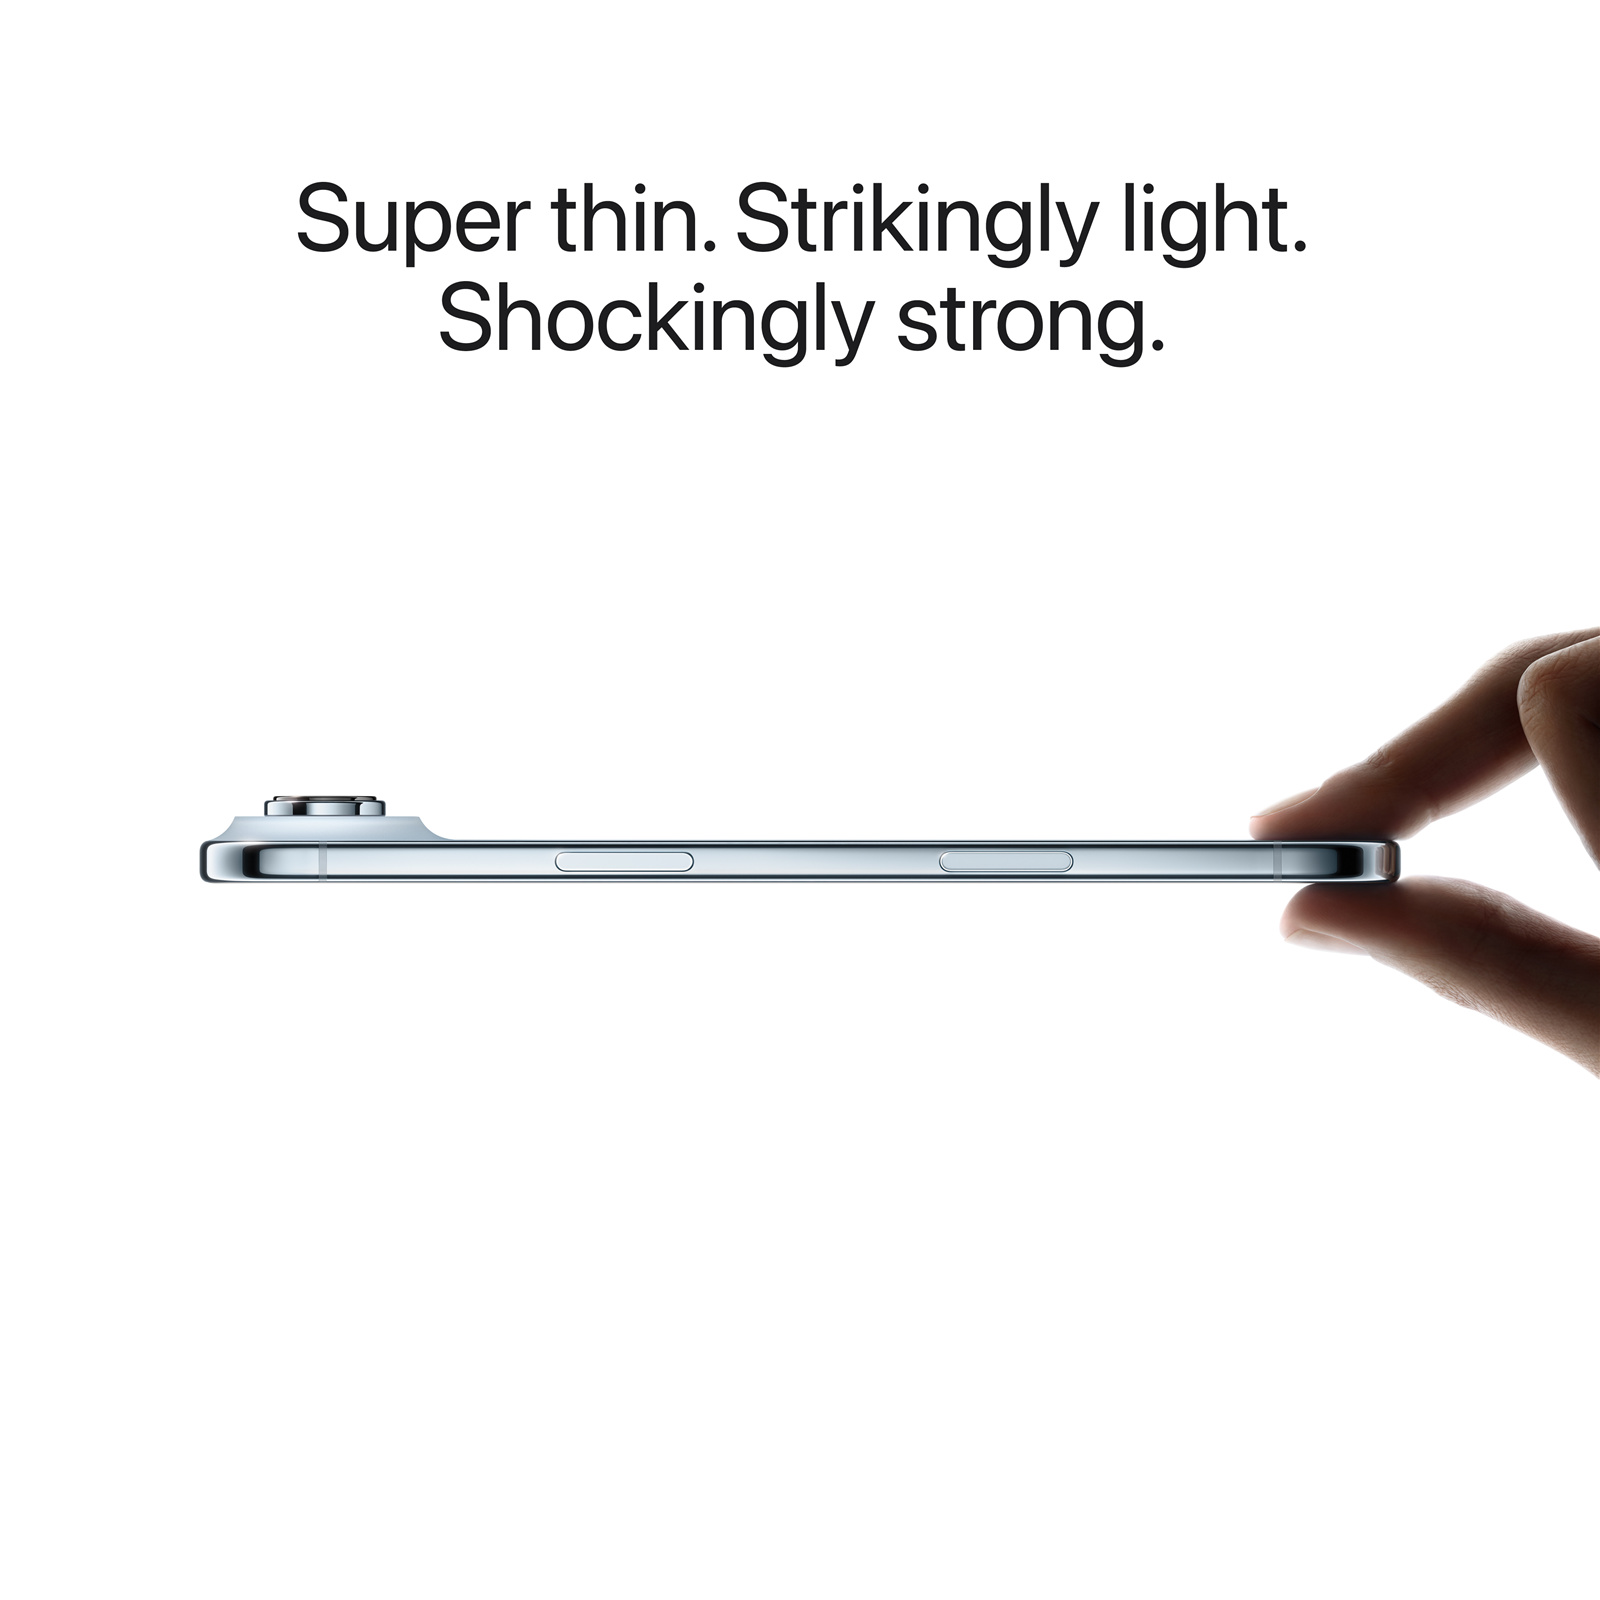
\includegraphics[width=0.5\textwidth]{imagenes/anuncio01.png}}
    \end{center}

    ¿Qué piensas después de ver este anuncio? \\
    \underline{\hspace{\linewidth}} \\
    \underline{\hspace{\linewidth}}

    \item A continuación se presenta un segundo anuncio.

    \begin{center}
        \fbox{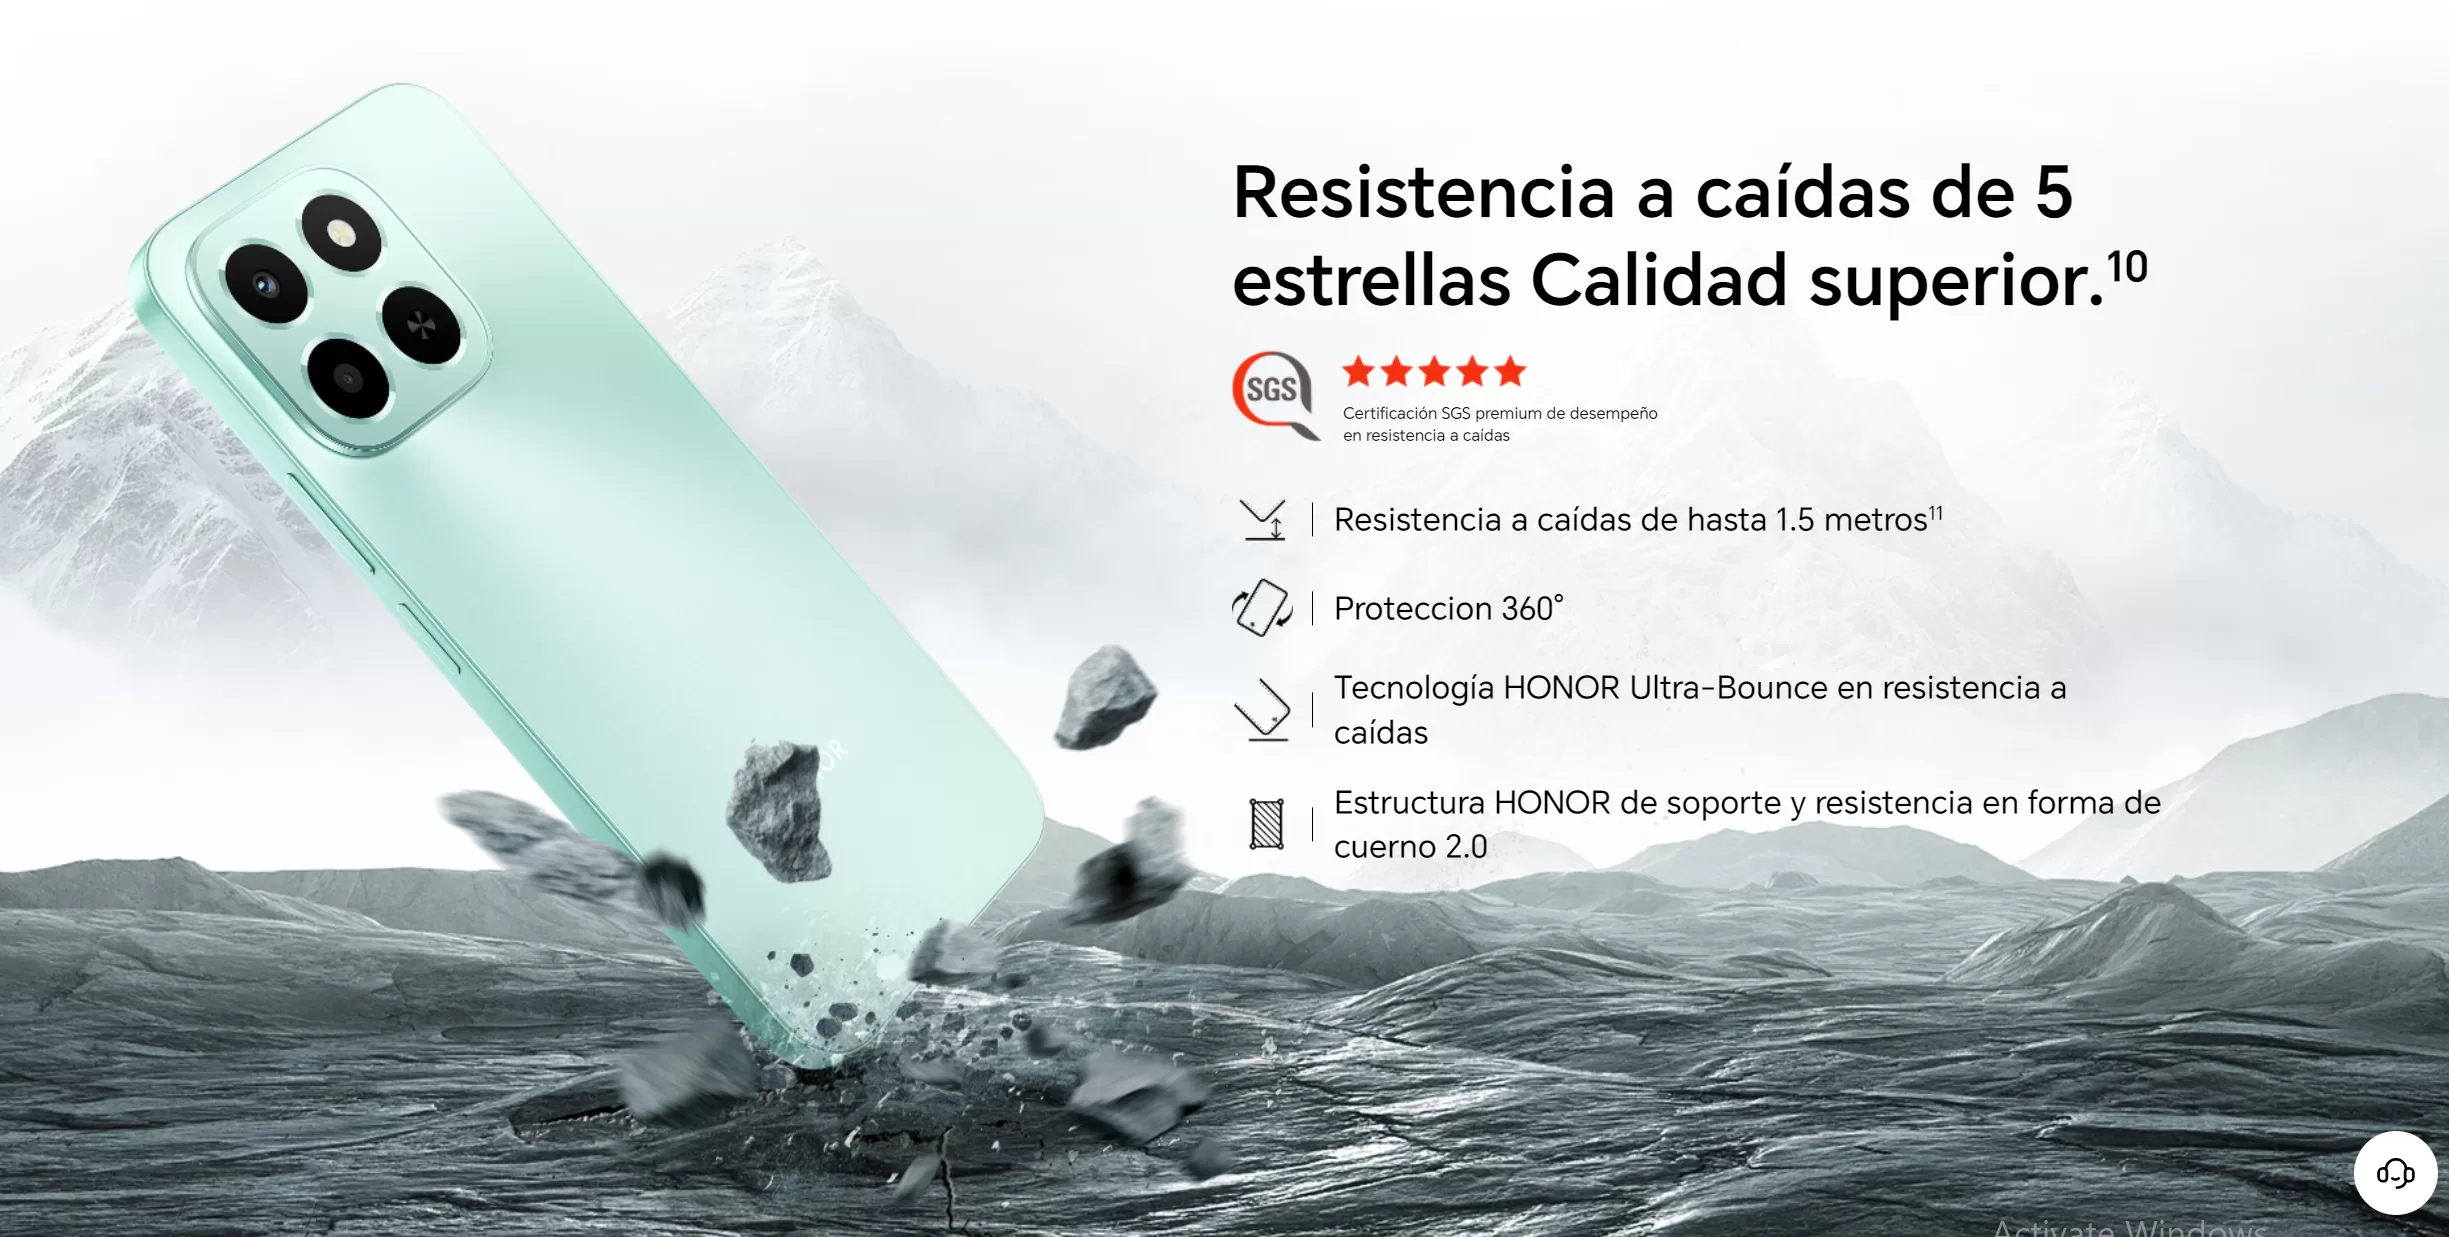
\includegraphics[width=0.8\textwidth]{imagenes/anuncio02.png}}
    \end{center}

    ¿Qué piensas o qué sensación te deja después de ver este anuncio? \\
    \underline{\hspace{\linewidth}} \\
    \underline{\hspace{\linewidth}}

\end{enumerate}

% ─── BLOQUE 5: Durabilidad y reparación ──────────────────────────────────────
\subsection*{Sección 5: Durabilidad, reparación y ciclo de vida}

\begin{enumerate}[resume]

    \item ¿Alguna vez te has preguntado por qué, después de aproximadamente 3 o
    4 años, sueles cambiar tus dispositivos electrónicos? \\
    \textbf{Sí} \quad \textbf{No}

    \item Pensando en el año 2011 —hace aproximadamente 15 años— y en cómo era
    el ritmo de vida y la resistencia de los dispositivos en esa época, ¿crees
    que actualmente las cosas están hechas para desecharse? \\
    \textbf{Sí} \quad \textbf{No}

    \item Imagina que tienes la oportunidad de comprar el teléfono que deseas,
    pero debes elegir entre dos opciones respecto a los materiales con los que
    fue fabricado: materiales con los estándares de calidad actuales o
    materiales con los estándares de hace 15 años. ¿Cuál elegirías? \\
    \textbf{Materiales actuales} \quad \textbf{Materiales de hace 15 años}

    \item ¿Cuáles son tus motivos para la respuesta anterior? \\
    \underline{\hspace{\linewidth}} \\
    \underline{\hspace{\linewidth}}

    \item Si tuvieras la opción de reparar tu teléfono inteligente o laptop
    —sabiendo que no quedaría en malas condiciones, que aumentaría su vida útil
    al menos dos años más, que se podría ampliar su memoria, que continuaría
    recibiendo actualizaciones y que el costo sería correspondiente únicamente a
    los materiales y la mano de obra— ¿elegirías repararlo o preferirías comprar
    uno nuevo? \\
    \textbf{Repararlo} \quad \textbf{Comprar uno nuevo}

    \item ¿Cuáles son tus motivos para la respuesta anterior? \\
    \underline{\hspace{\linewidth}} \\
    \underline{\hspace{\linewidth}}

    \item ¿Qué tanto te importa adquirir lo que está de novedad o es lo más
    popular en el mercado? \\
    \textbf{Me importa mucho} \quad \textbf{Me importa un poco} \quad \textbf{No
    me importa}

    \item En caso de que te importe mucho o un poco, ¿cuáles son tus razones
    para querer adquirir productos nuevos cuando los tuyos funcionan
    correctamente? \\
    \underline{\hspace{\linewidth}} \\
    \underline{\hspace{\linewidth}}

\end{enumerate}

% ─── BLOQUE 6: Utilidad de herramienta propuesta ──────────────────────────────────────
\subsection*{Sección 6: Percepción de utilidad de la herramienta propuesta}

\begin{enumerate}[resume]

    \item Cuando vas a comprar un dispositivo electrónico, ¿qué tan difícil 
    te resulta encontrar información clara y confiable sobre el producto?
    
    \textbf{Muy difícil} \quad \textbf{Algo difícil} \quad \textbf{Poco difícil} \quad \textbf{Nada difícil}

    \item Al momento de comprar un dispositivo electrónico, ¿consultas 
    opiniones de otros usuarios antes de tomar tu decisión?
    
    \textbf{Siempre} \quad \textbf{A veces} \quad \textbf{Casi nunca} \quad \textbf{Nunca}

    \item ¿Alguna vez has dejado de comprar un producto porque no encontraste 
    suficiente información confiable sobre él?
    
    \textbf{Sí} \quad \textbf{No}

    \item Imagina una aplicación que, al escanear el código de barras de un 
    dispositivo electrónico, te muestre de forma clara y progresiva: 
    información del fabricante, opiniones de usuarios reales, 
    certificaciones de sostenibilidad y opciones de reparación cercanas 
    a tu ubicación. ¿Qué tan útil considerarías esta herramienta?
    
    \textbf{Muy útil} \quad \textbf{Útil} \quad \textbf{Poco útil} \quad \textbf{Nada útil}

    \item ¿Crees que contar con una herramienta como la descrita anteriormente 
    influiría en tu decisión de compra?
    
    \textbf{Definitivamente sí} \quad \textbf{Probablemente sí} \quad 
    \textbf{Probablemente no} \quad \textbf{Definitivamente no}

    \item ¿Utilizarías una aplicación de este tipo antes de adquirir 
    un dispositivo electrónico?
    
    \textbf{Sí} \quad \textbf{No} \quad \textbf{Tal vez}

\end{enumerate}

\noindent Te agradecemos el tiempo brindado y las respuestas proporcionadas, éstas serán
usadas para poder fundamentar nuestra investigación, si estás interesade en
leerla no dudes en decirnos y cuando haya sido completada te la proporcionamos. 

\noindent Recuerda que para que el mundo cambie debes de cuestionar todo lo que haces y
sobre todo lo que te dicen, nosotros tenemos el poder como consumidores de
cambiar el rumbo. 
\newpage

\newpage

\end{document}
